\section{Problem Set 6}

\subsection{Continuous Control Law}

\subsubsection{Control Method Considerations}

The control method considerations are the same as in Section \ref{sec:control_objectives} and Section \ref{sec:control_considerations}. Our system has four distinct operational modes, each with their own unique control accuracy and safety requirements. We also have control considerations for the maneuvers for transitioning between different modes. In this section, we utilize a continuous control input rather than impulse delta-v inputs.

To provide enough time for the continuous control to act effectively, we increased the duration of each mode (maneuver times and station keeping times between maneuvers), provided in Table \ref{tab:mode_durations_cont}.

\begin{table}[h!]
\centering
\begin{tabular}{|c|c|}
\hline
\textbf{Phase} & \textbf{Number of Orbits} \\
\hline
Mode 2 & 15 \\
Station-Keeping 2 & 5 \\
Mode 3 & 10 \\
Station-Keeping 3 & 5 \\
Mode 4 & 10 \\
Station Keeping 4 & 5 \\
\hline
\end{tabular}
\caption{Number of orbits spent in each mode and station-keeping phase} \label{tab:mode_durations_cont}
\end{table}

Our system is still working in a near-circular orbit with two deputy spacecraft. The "Watcher/SV2" spacecraft only performs station-keeping, whereas the "Docker/SV3" performs various maneuvers to dock with the chief spacecraft. Table \ref{tab:mode_control_methods_cont} is analogous to Table \ref{tab:mode_control_methods}, but with continuous control methods considered.


\definecolor{lightgray}{gray}{0.9}

\begin{table}[H]
    \centering
    \caption{Control Methods by Mode of Operation}
    \renewcommand{\arraystretch}{1.3}

    \begin{tabularx}{\textwidth}{|>{\raggedright\arraybackslash}p{0.13\textwidth}|%
                                      >{\raggedright\arraybackslash}p{0.13\textwidth}|%
                                      >{\raggedright\arraybackslash}p{0.12\textwidth}|%
                                      >{\raggedright\arraybackslash}p{0.12\textwidth}|%
                                      >{\raggedright\arraybackslash}p{0.12\textwidth}|%
                                      >{\raggedright\arraybackslash}X|}
        \rowcolor{lightgray}
        \hline
        \textbf{Mode of Operation} & \textbf{Tracked State} & \textbf{In-plane Control Method} & \textbf{Out-of-plane Control Method} & \textbf{Control Window} & \textbf{Reasoning} \\
        \hline
        General Station Keeping (SV2 always and SV3 Mode 1) & Relative orbital elements that provide passive safety & Along-track continuous control input & Cross-track continuous control input & Full duration of station-keeping (see Table \ref{tab:mode_durations}) & Very small control inputs to maintain position when needed. \\
        \hline
        Approach Transfer (SV3 Mode 2) & Desired Mode 2 final ROE & Along-track continuous control input & Cross-track continuous control input & 15 orbits for maneuver & Using Lyapunov-based control scheme with modifications for handling $\delta \lambda $ drift\\
        \hline
        Proximity Maneuvers (SV3 Mode 3) & Desired Mode 3 final ROE & Along-track continuous control input & Cross-track continuous control input & 15 orbits for maneuver & Using Lyapunov-based control scheme with modifications for handling $\delta \lambda $ drift\\
        \hline
        Docked Station Keeping (SV3 Mode 4) & N/A (Docked State) & No in-plane control & No out-of-plane control & Service duration & Rigid-body docking eliminates relative motion; no active control required. \\
        \hline
    \end{tabularx}
    \label{tab:mode_control_methods_cont}
\end{table}


\subsubsection{Lyapunov Control Implementation}\label{sec:Lyapunov_implementation}
Although we had the different ideas for control methodologies for the different modes, during the duration of this submission we were only able to get one method working exactly to meet our requirements: Lyapunov control without constraints. 

First, the state-space reduced model as described by Steindorf is considered \cite{steindorf2017constrained}. Since tangential thrusts are two times more efficient than radial thrusts in changing $\delta e$ and $\delta a$, the reduced model does not involve any radial thrusts. Thus, the ROE vector is reduced to exclude $\delta \lambda$, since it can only be controlled directly by radial thrusts.Note that $\delta \lambda$ can still be controlled by adjusting $\delta a$ to induce a Keplerian drift such that $\delta \lambda$ reaches a desired state at the end of the control window. This process will be desribed in full later. The reduced ROE vector is defined as: 
\begin{align*}
\delta \bm{\alpha} = \begin{bmatrix} \delta a, \delta e_x, \delta e_y, \delta i_x, \delta i_y \end{bmatrix}^\top
\end{align*}

From here the reduced state-space model can be defined as follows:
\begin{equation}
\begin{bmatrix}
\delta \dot{\bm{\alpha}} \\
\delta \ddot{a}
\end{bmatrix}
=
A
\begin{bmatrix}
\delta \bm{\alpha} \\
\delta \dot{a}
\end{bmatrix}
+
\begin{bmatrix}
B \\
\bm{0}_{1 \times 3}
\end{bmatrix}
\bm{u}
\label{eq:reduced_state_space}
\end{equation}

The reduced ROE state is augmented by the differential rate of change of the relative semi-major-axis, $\delta \dot{a}$. This is to  deal with aerodynamic drag, but that is neglected in our case. 

The plant matrix for the reduced model with J2 effects is given by:
\begin{equation}
A_{J2}(\bm{\alpha}_c) = \kappa
\begin{bmatrix}
0 & 0 & \frac{7}{2} e_y Q & -4 e_x e_y G Q & -(1 + 4 e_y^2 G) Q & 5 e_y S & 0 & 0 \\
0 & 0 & -\frac{7}{2} e_x Q & (1 + 4 e_x^2 G) Q & 4 e_x e_y G Q & -5 e_x S & 0 & 0 \\
0 & 0 & 0 & 0 & 0 & 0 & 0 & 0 \\
0 & 0 & \frac{7}{2} S & -4 e_x G S & -4 e_y G S & 2 T & 0 & 0 \\
0 & 0 & 0 & 0 & 0 & 0 & 0 & 0 \\
\end{bmatrix}
\end{equation} \label{eq:continuous_control_A}
\noindent where
\[
\dot{\omega} = \kappa Q; \qquad \gamma = \frac{3}{4} J_2 R_e^2 \sqrt{\mu}; \qquad \eta = \sqrt{1 - e^2}; \qquad \kappa = \frac{\gamma}{a_c^{7/2} \eta_c^4}
\]

\[
e_x = e_c \cos(\omega_c); \qquad e_y = e_c \sin(\omega_c); \qquad E = 1 + \eta_c; \qquad F = 4 + 3 \eta_c; \qquad G = \frac{1}{\eta_c^2}
\]

\[
P = 3 \cos(i_c)^2 - 1; \qquad Q = 5 \cos(i_c)^2 - 1; \qquad S = \sin(2 i_c); \qquad T = \sin(i_c)^2
\]

The control input matrix for the reduced model is given by:

\begin{equation}
\bm{B}(\bm{\alpha}_c) = \frac{1}{a n}
\begin{bmatrix}
\frac{2}{\eta}(1 + e \cos f) & 0 \\
\eta \frac{(2 + e \cos f) \cos \theta + e_x}{1 + e \cos f} & \frac{\eta e_y}{\tan i} \cdot \frac{\sin \theta}{1 + e \cos f} \\
\eta \frac{(2 + e \cos f) \sin \theta + e_y}{1 + e \cos f} & -\frac{\eta e_x}{\tan i} \cdot \frac{\sin \theta}{1 + e \cos f} \\
0 & \eta \frac{\cos \theta}{1 + e \cos f} \\
0 & \eta \frac{\sin \theta}{1 + e \cos f}
\end{bmatrix}
\end{equation} \label{eq:continuous_control_B}

where \( f \) is the true anomaly and \( \theta = f + \omega \).

And the control input is given by:
\begin{equation}
\bm{u} = \begin{bmatrix} u_t, u_n \end{bmatrix}^\top
\end{equation}
which represents the control acceleration in along-track and normal directions of the co-rotating RTN frame.

For continuous control, a feedback controller can be implemented to stabilize the system at a desired reference, $\delta \boldsymbol{\alpha}_a$. A control law that ensures the relative state to asymptotically tend towards the desired reference is given by: 

\begin{equation}
\mathbf{u} = -\mathbf{B}^* \left[ A \delta \boldsymbol{\alpha} + P \left( \delta \boldsymbol{\alpha} - \delta \boldsymbol{\alpha}_a \right) \right]
\label{eq:feedback_continuous}
\end{equation}

To ensure that this control law achieves asymptotic stability, a Lyapunov function which is positive definite and whose time derivative is negative definite is chosen. Let the reduced state-space system described by Equation \ref{eq:reduced_state_space} be subject to the control law given in Equation \ref{eq:feedback_continuous} with $P$ being positive definite. A Lyapunov function candidate is given by:

\begin{equation}
V(\delta \boldsymbol{\alpha}_a, \delta \boldsymbol{\alpha}) = \frac{1}{2} (\delta \boldsymbol{\alpha} - \delta \boldsymbol{\alpha}_a)^\top (\delta \boldsymbol{\alpha} - \delta \boldsymbol{\alpha}_a) 
= \frac{1}{2} \Delta \boldsymbol{\alpha}^\top \Delta \boldsymbol{\alpha}
\label{eq:Lyapunov_candidate}
\end{equation}

By taking the derivative of Equation \ref{eq:Lyapunov_candidate} and substituting Equation \ref{eq:feedback_continuous} into Equation \ref{eq:Lyapunov_candidate}, it can be proven that Equation \ref{eq:Lyapunov_candidate} is a Lyapunov function:

\begin{align}
\dot{V}(\delta \boldsymbol{\alpha}_a, \delta \boldsymbol{\alpha}) 
&= \Delta \boldsymbol{\alpha}^\top \Delta \dot{\boldsymbol{\alpha}} \notag \\
&= \Delta \boldsymbol{\alpha}^\top \left( \dot{\delta \boldsymbol{\alpha}} - \dot{\delta \boldsymbol{\alpha}}_a \right) \notag \\
&= \Delta \boldsymbol{\alpha}^\top \left( A(\alpha_c) \delta \boldsymbol{\alpha} + B(\alpha_c) \mathbf{u} - 0 \right) \notag \\
&= \Delta \boldsymbol{\alpha}^\top \left( A(\alpha_c) \delta \boldsymbol{\alpha} + B(\alpha_c) \left( -\mathbf{B}^* \left[ A \delta \boldsymbol{\alpha} + P(\delta \boldsymbol{\alpha} - \delta \boldsymbol{\alpha}_a) \right] \right) \right) \notag \\
&= -\Delta \boldsymbol{\alpha}^\top P \Delta \boldsymbol{\alpha}
\tag{4.3}
\end{align}

which is negative definite.

The matrix \( P \) is defined as:

\[
P = \frac{1}{k} \begin{bmatrix}
\cos(J)^N & 0 & 0 & 0 & 0 \\
0 & \cos(J)^N & 0 & 0 & 0 \\
0 & 0 & \cos(J)^N & 0 & 0 \\
0 & 0 & 0 & \cos(H)^N & 0 \\
0 & 0 & 0 & 0 & \cos(H)^N \\
\end{bmatrix}
\]

where \( k \in \mathbb{R}^{+} \) is an arbitrary large scaling scalar, 
\( J = u - \bar{u}_{ip} \), \( H = u - \bar{u}_{oop} \), and 
\( u = M + \omega \) is the mean argument of latitude. 
The exponent \( N \in \mathbb{N} \) such that \( N \bmod 2 = 0 \land N > 2 \) 
defines to which extent the control inputs are centered around the fuel optimal locations to control the in-plane \((\delta a, \delta e)\) motion at \( \bar{u}_{ip} \), and the out-of-plane \((\delta i)\) motion at \( \bar{u}_{oop} \).

The optimal locations for near-circular orbits to apply thrust are given by:

\[
\bar{u}_{ip} = \text{atan2} \left( \Delta \delta e_y, \Delta \delta e_x \right)
\]
\[
\bar{u}_{oop} = \text{atan2} \left( \Delta \delta i_y, \Delta \delta i_x \right)
\]

The parameters $N$ and $k$ are used to tune the controller response. 

\textbf{\textit{Indirect Control of $\delta\lambda$}}

Direct control of $\delta \lambda$ would require the additional degree of freedom of radial burns, which can be very inefficient for $\Delta v$ usage. Instead, $\delta \lambda$ can be corrected indirectly by using along-track burns and applying an intermediate $\delta a_{des}$, and allowing for Keplerian dynamics to drift $\delta \lambda$ by a desired amount. \cite{steindorf2017constrained}

The rate of change of the $\delta \lambda$ is based on the semi-major axis separation $\delta a$
\begin{align}
    \delta \dot{\lambda} = -\frac{3}{2}n_c \delta a 
\end{align}
We can thus modulate the $\delta a_{des}$ such that we can help converge $\delta \lambda$ to zero by the end of the maneuver period. We can thus set up a desired $\delta \dot{\lambda}$ that helps converge $\Delta \delta \lambda \rightarrow 0$
\begin{equation}
\delta \dot{\lambda}_a =
\begin{cases}
-\min \left\{ \left| \frac{\Delta \delta \lambda}{\tau} \right| , \delta \dot{\lambda}_{\text{ref}} \right\}, & \text{if } \Delta \delta \lambda \geq 0 \\
\phantom{-}\min \left\{ \left| \frac{\Delta \delta \lambda}{\tau} \right| , \delta \dot{\lambda}_{\text{ref}} \right\}, & \text{if } \Delta \delta \lambda < 0
\end{cases}
\end{equation}

We determine those upper bounds $\delta \dot{\lambda}_{ref}$ based on a $\delta a_{ref}$
\begin{align}
    \delta \dot{\lambda}_{ref} = -\frac{3}{2} n_c \delta a_{ref}
\end{align}

where $\delta a_{ref}$ accounts for the shift in $\delta a$ that occurs when performing tangential burns to modify the in-plane eccentricity vector change $\Delta \delta \textbf{e}$. We thus use the following expression for $\delta a_{ref}$ as
\begin{align}
    \delta a_{ref} &= \left|\frac{1}{a_cn_c \eta}(1 + e \cos(f))\cdot  \frac{v_{opt}}{2\cdot n_{orbits}}\right| \\
    v_{opt} &= \frac{a_cn_c||\Delta\delta \textbf{e}||_2}{2\eta}
\end{align}

With this, we now have all the information required to calculate $\delta \dot{\lambda}_a $, from which we can calculate the new target $\delta a_a$ that we should have the Lyapunov controller track to cause the desired shift in $\delta \lambda$.
\begin{align}
    \delta a_a = -\frac{2}{3}\frac{\delta \dot{\lambda}_a}{n_c}
\end{align}
This is then utilized as an intermediary reference $\delta a$. The new $\Delta \delta a = \delta a - \delta a_a$, rather than using a reference of $\delta a_a = 0$.

There is an additional accomodation made to the matrix P to bound the maximum tracking error to be around $\delta a_{ref}$, to prevent the tracking error from increasing to an amount that then conflicts with the control burn required for eccentricity vector correction. The adjustment to matrix P is just setting terms to $0$ to stop feedback of any tracking error that gets larger than $\delta a_{ref}$.

\[
P_{|\delta a_a| \geq |\delta a_{ref}|} = \frac{1}{k} \begin{bmatrix}
0 & 0 & 0 & 0 & 0 \\
0 & 0 & 0 & 0 & 0 \\
0 & 0 & 0 & 0 & 0 \\
0 & 0 & 0 & \cos(H)^N & 0 \\
0 & 0 & 0 & 0 & \cos(H)^N \\
\end{bmatrix}
\]

\subsubsection{Justificiation and Implementation of Control}

\textbf{\textit{Dynamics Model for Ground Truth Simulation}}

For our ground-truth simulation model, we utilized a FODE simulation model that is described in Section \ref{sec:fode_simulation} (utilizing RK4). This model gives us a high-fidelity model in which it is simple to incorporate J2 perturbations and drag models (although the drag models have not been implemented yet). The states of the satellites are stored and propagated in ECI co-ordinates. 

Based on the time-index of the simulation, it is decided whether station-keeping or maneuevering to the specified ROEs of the next mode is required. Then, the lyapunov control scheme is utilized to calculate required acceleration control inputs in the tangential and normal directions. These are then applied as an approximate change in velocity to the ECI state vector being propagated. The full structure of this code is shown in Algorithm \ref{alg:continuous_control_sim}
\begin{align}
    \Delta v_t = u_t \Delta t
\end{align}

\begin{algorithm}[H]
\caption{FODE Simulation with Continuous Control}
\begin{algorithmic}[1]

\State Initialize time array, chief semi-major axis, and empty state histories
\State Get maneuver control block times
\State Extract nominal ROE for SV2 and SV3

\For{each time step $t_i$ in $t_{\text{series}}$}
    \State Propagate SV1, SV2, SV3 states using RK4
    \State Convert SV2 and SV3 states to ROE w.r.t. SV1

    \State Compute control input to station-keep SV2
    \If{$t_i$ belongs to a maneuver block}
        \State Get desired final ROE values for SV3
        \State Compute control input to maneuver SV3
    \Else
        \State Compute control input to station-keep SV3
    \EndIf
    \State Convert control inputs to a change in $\Delta v$ in the ECI frame
    \State Apply control input
\EndFor
\State Convert SV2 and SV3 final states to RTN position relative to SV1
\State Plot desired data in RTN and ROE frames.
\EndProcedure
\end{algorithmic}
\end{algorithm} \label{alg:continuous_control_sim}

\textbf{\textit{Selection of Dynamics Model for Continuous Controller}} \\
The Lyapunov-based control uses a reduced-order model as an approximation of the true dynamics that can be utilized for control design. This reduced order model is captured in the $A$ and $B$ matrices provided in Equation \ref{eq:continuous_control_A} and \ref{eq:continuous_control_B}. Control maneuvers calculate a control input $u_t$ in the RTN frame (which is converted to ECI when being applied to FODE states), and the input and reference ROEs use quasi-nonsingular relative orbital elements.

\textbf{\textit{Actuator Implementation, Sensor and Disturbance Models}} \\
For this submission, considerations of the delta-v budget, actuator implementation, sensor models, and disturbance models (apart from J2) are ignored. These other practical considerations will be incorporated in future submissions.

\subsubsection{Results and Analysis of Continuous Control Performance} \label{sec:analysis_of_control_cont}

The results of the Lyapunov-based unconstrained continuous control scheme are shown in the following figures. These plots include all modes of the Watcher (SV2) and Docker (SV3) satellites, which involve maneuvers between desired ROEs and station-keeping.

Figures \ref{fig:cont_control_RT}, \ref{fig:cont_control_RN}, and \ref{fig:cont_control_NT} show all the control modes in the RTN frame. Significant drifts in the tangential and normal directions are observed, but are also corrected for by the control system. This behavior will be explored further in subsequent figures.

\begin{figure}[H]
    \centering
    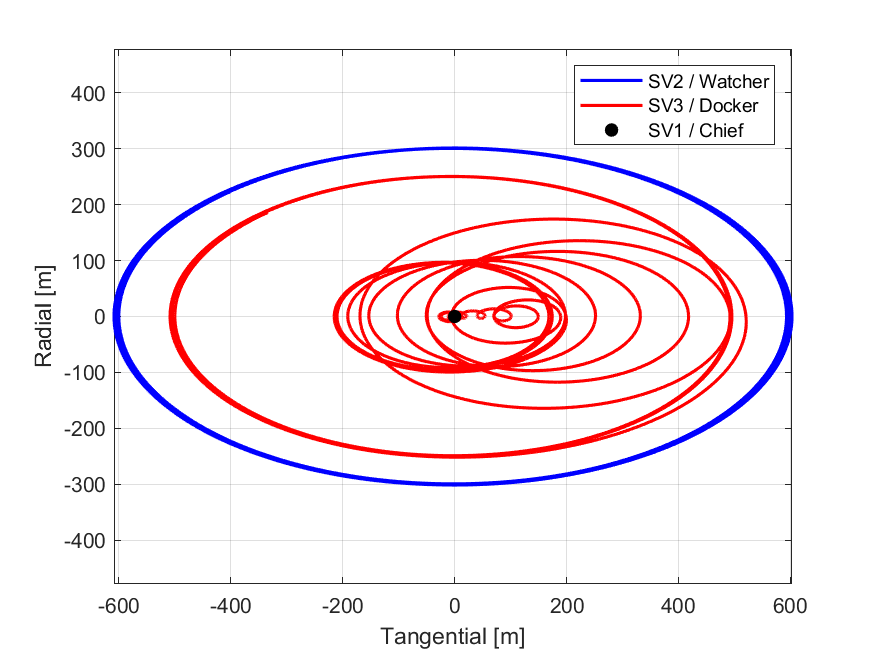
\includegraphics[width=0.5\linewidth]{sim/figures/PS6/RTN_3d_projections_all_maneuvers_cont.png_RT.png}
    \caption{Continuous control modes in RT plane}
    \label{fig:cont_control_RT}
\end{figure}
\begin{figure}[H]
    \centering
    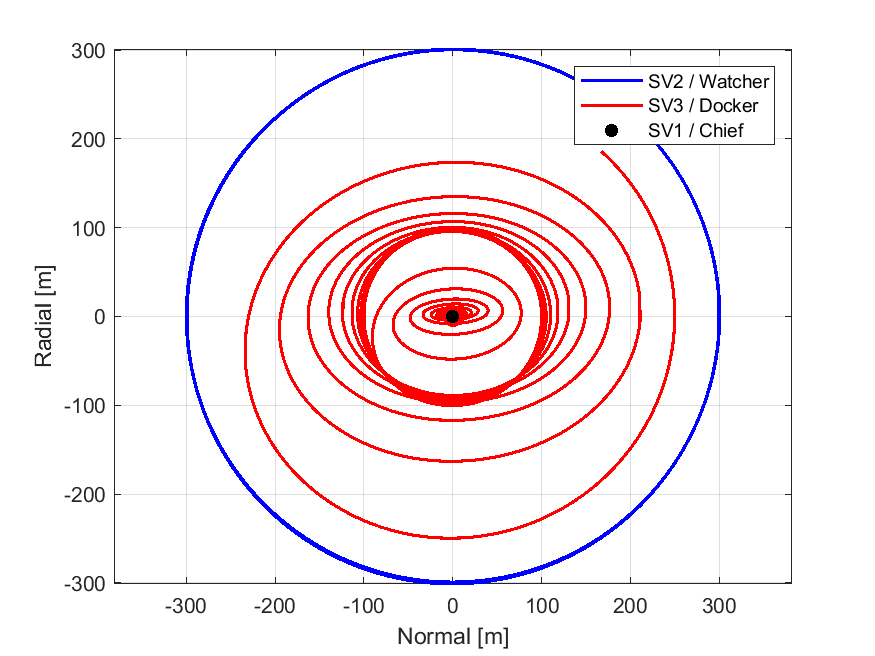
\includegraphics[width=0.5\linewidth]{sim/figures/PS6/RTN_3d_projections_all_maneuvers_cont.png_RN.png}
    \caption{Continuous control modes in RN plane}
    \label{fig:cont_control_RN}
\end{figure}
\begin{figure}[H]
    \centering
    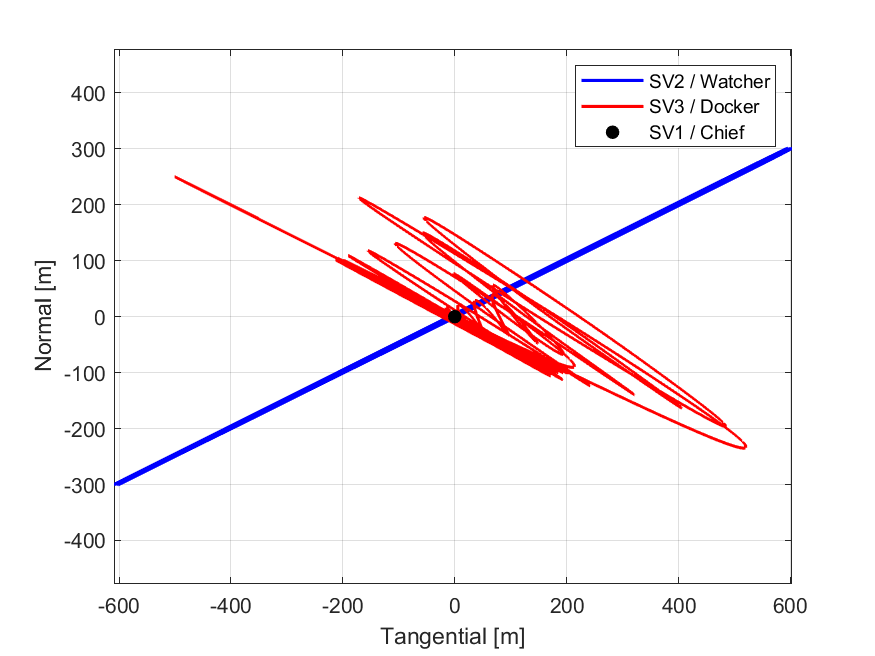
\includegraphics[width=0.5\linewidth]{sim/figures/PS6/RTN_3d_projections_all_maneuvers_cont.png_NT.png}
    \caption{Continuous control modes in NT plane}
    \label{fig:cont_control_NT}
\end{figure}

For SV2, Figures \ref{fig:roe_planes_modes_cont_SV2} and \ref{fig:roe_time_modes_cont_SV2} show the desired and actual ROEs for each mode, which remain constant. The control system tries to keep all ROEs at their initial value. It does so fairly successfully as all ROEs end up within 1 meter of their desired value. These offsets are introduced due to the control system trying to keep $\delta \lambda$ as close to zero as possible through changing $\delta a$ as explain in Section \ref{sec:Lyapunov_implementation}. This has follow on effects on the relative eccentricity and inclination, although they are minor. 

\begin{figure}[H]
    \centering
    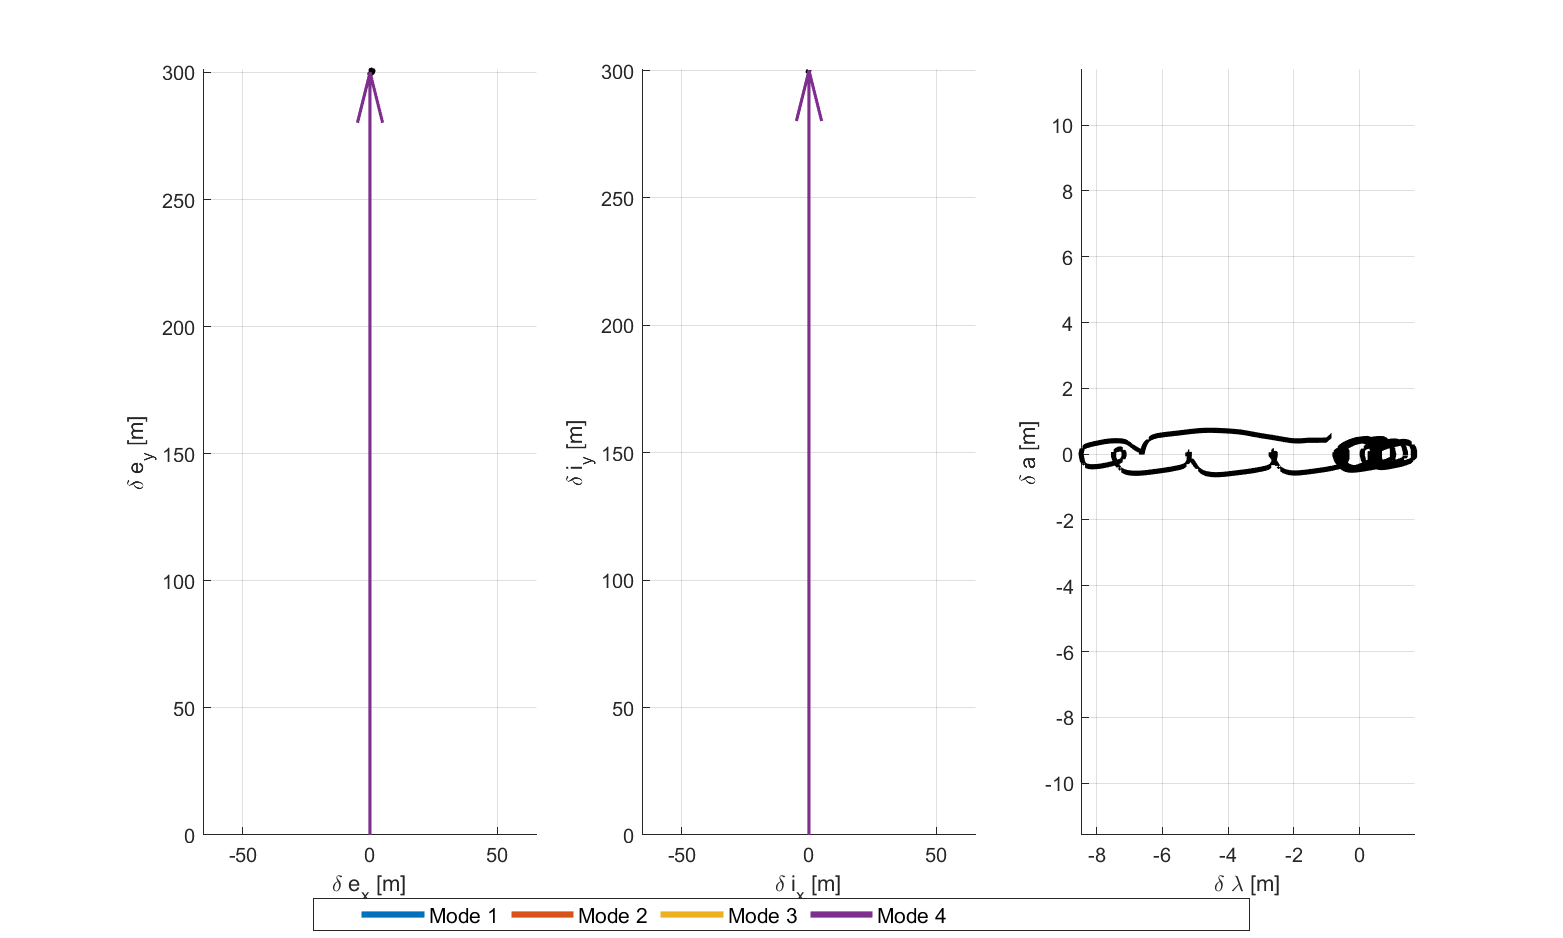
\includegraphics[width=0.75\linewidth]{sim/figures/PS6/ROE_planes_modes_SV2.png}
    \caption{Actual and desired ROE plotted for all modes in ROE planes, SV2}
    \label{fig:roe_planes_modes_cont_SV2}
\end{figure}
\begin{figure}[H]
    \centering
    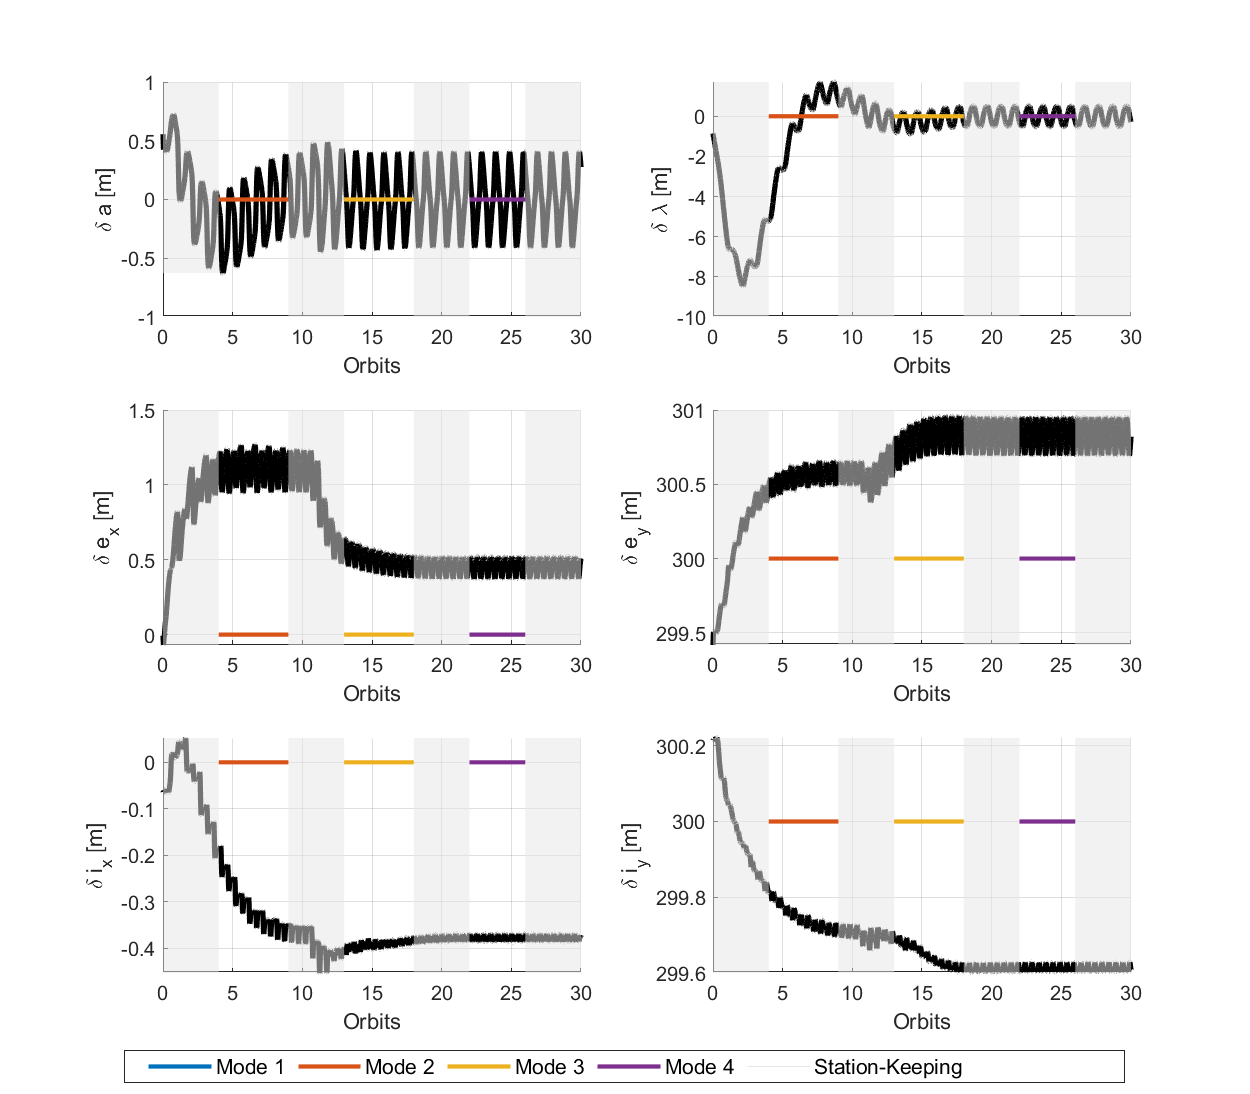
\includegraphics[width=0.75\linewidth]{sim/figures/PS6/ROE_over_time_modes_SV2.png}
    \caption{Actual and desired ROE plotted for all modes in ROE time history, SV2}
    \label{fig:roe_time_modes_cont_SV2}
\end{figure}

The same trends can be seen in the errors plotted in Figure \ref{fig:roe_error_time_modes_cont_SV2}. 
\begin{figure}[H]
    \centering
    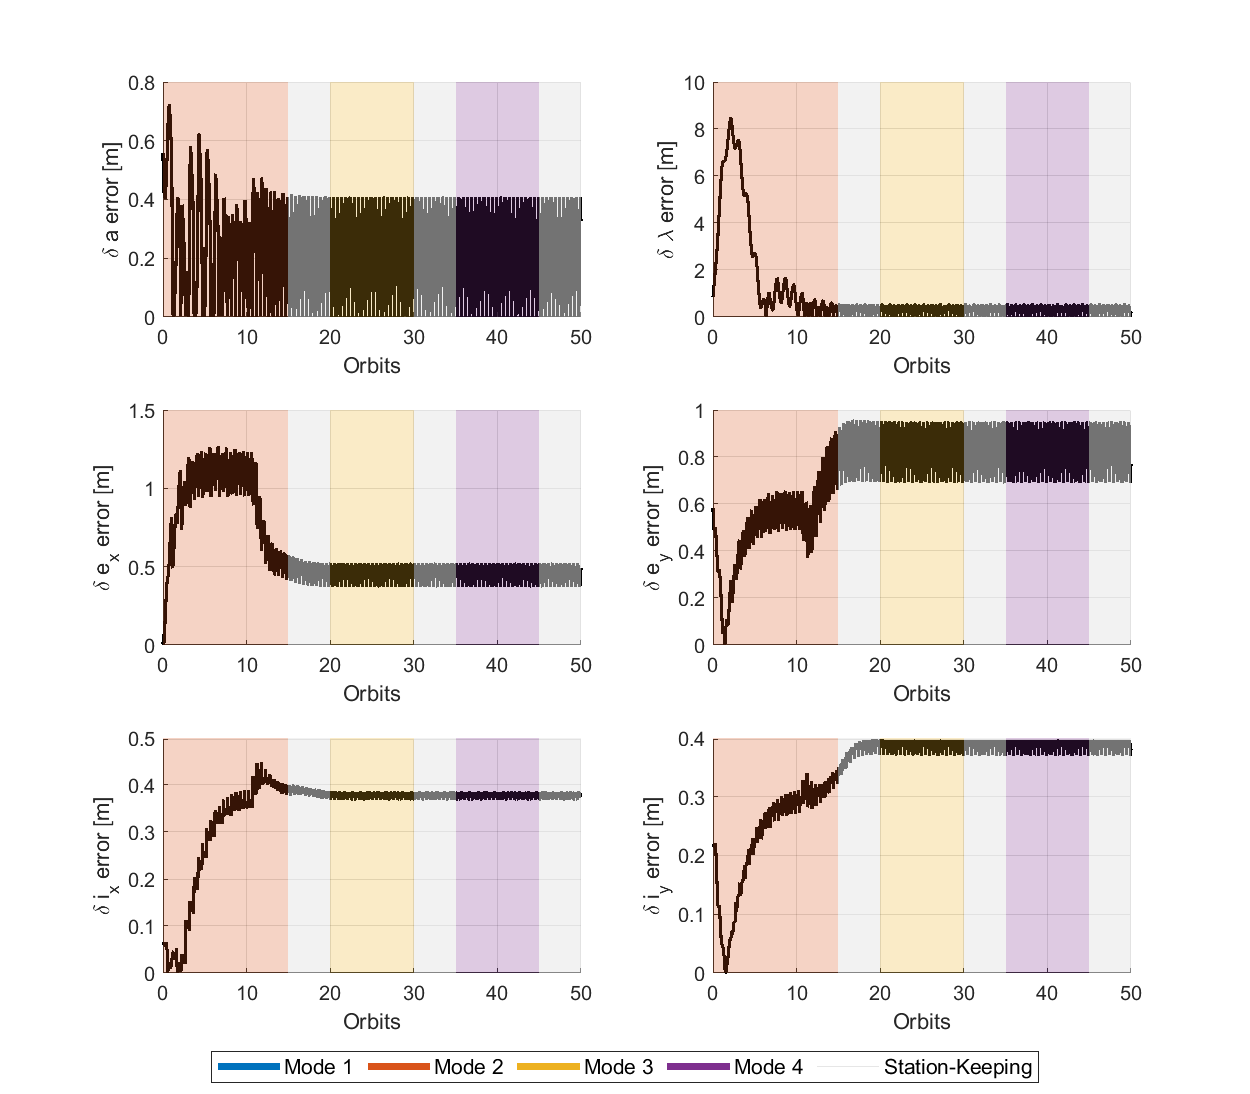
\includegraphics[width=0.75\linewidth]{sim/figures/PS6/ROE_error_over_time_modes_SV2.png}
    \caption{Tracking error between actual and desired ROE plotted for all modes in ROE time history, SV2}
    \label{fig:roe_error_time_modes_cont_SV2}
\end{figure}

For SV3, Figures \ref{fig:roe_planes_modes_cont_SV3} and \ref{fig:roe_time_modes_cont_SV3} show the desired and actual ROEs for each mode. $\delta a$ becomes non-zero during the maneuvers because there are along-track elements. The magnitude of $\delta a$ is chosen in order to induce a calculated rate of change in $\delta \lambda$ so that it too can reach a desired value. So $\delta \lambda$ also becomes non-zero during maneuvers, but converges back to zero by the end of the maneuver. This indirect control method is explained at the end of Section \ref{sec:Lyapunov_implementation}. 

$\delta e_x$ and $\delta i_x$ are always meant to be zero, but again the maneuvers introduce variations. Each control mode tries to return $\delta e_x$ and $\delta i_x$ to zero but is unable to get all the way there. These errors can be addressed by allowing for more orbits to converge and more robust station-keeping control in between modes. Right now the continuous station-keeping control is designed to hold the state that it is started at. 

$\delta e_y$ and $\delta i_y$ exhibit the most accurate behavior. The control system is able to reach the desired $\delta e_y$ and $\delta i_y$ in each mode with very little error. This is important because these are the only non-zero factors in the desired ROEs and drive passive safety. 

\begin{figure}[H]
    \centering
    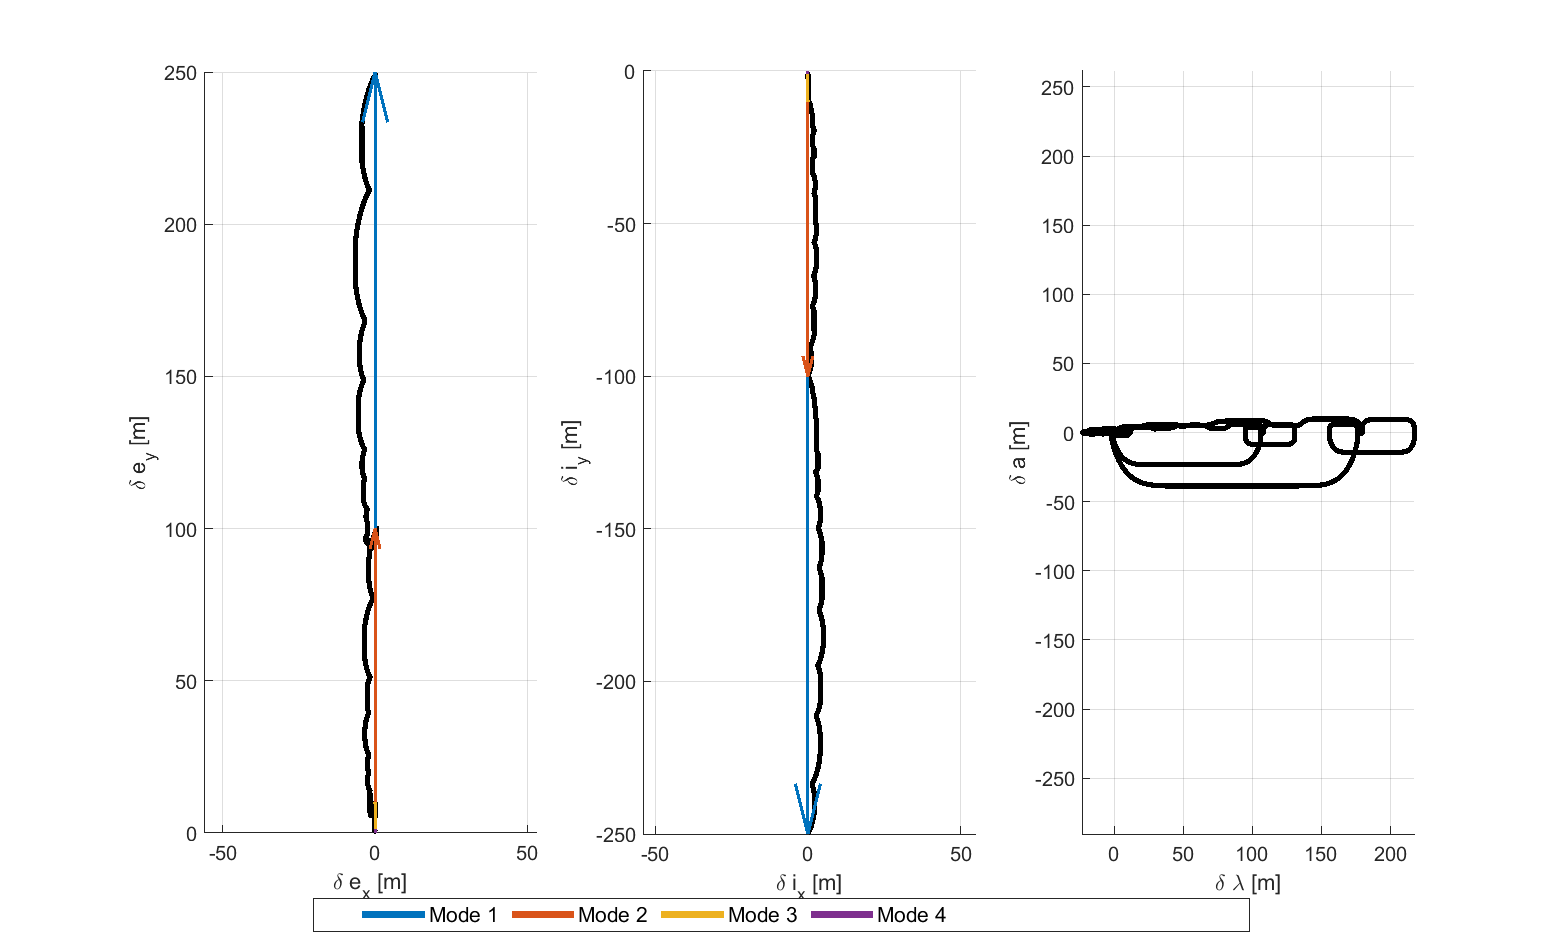
\includegraphics[width=0.75\linewidth]{sim/figures/PS6/ROE_planes_modes_SV3.png}
    \caption{Actual and desired ROE plotted for all modes in ROE planes, SV3}
    \label{fig:roe_planes_modes_cont_SV3}
\end{figure}
\begin{figure}[H]
    \centering
    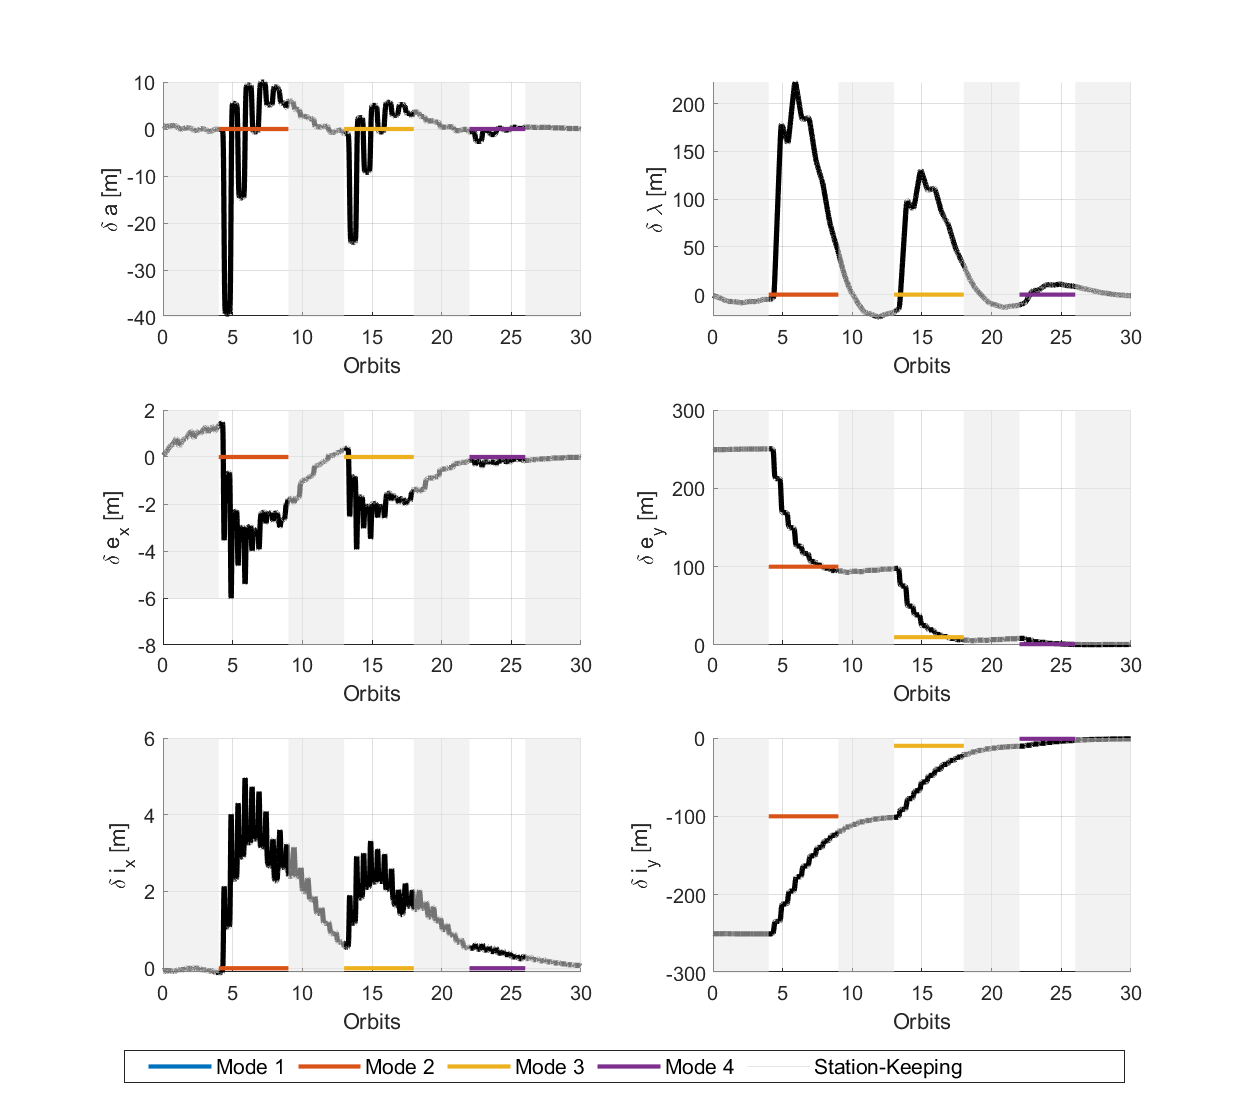
\includegraphics[width=0.75\linewidth]{sim/figures/PS6/ROE_over_time_modes_SV3.png}
    \caption{Actual and desired ROE plotted for all modes in ROE time history, SV3}
    \label{fig:roe_time_modes_cont_SV3}
\end{figure}

Figure \ref{fig:roe_error_time_modes_cont_SV3} reflects the same behavior in the tracking errors. The control system is able to track all of the desired ROEs very well. The remaining tracking errors can be mitigated either through allowing for more time to converge, adjusting values of $k$ and $N$, or an enhanced station-keeping method. Other methods, such as Lyapunov with constraints or convex optimization, can also be explored, but do not appear to be necessary for the desired behavior in this system. 

\begin{figure}[H]
    \centering
    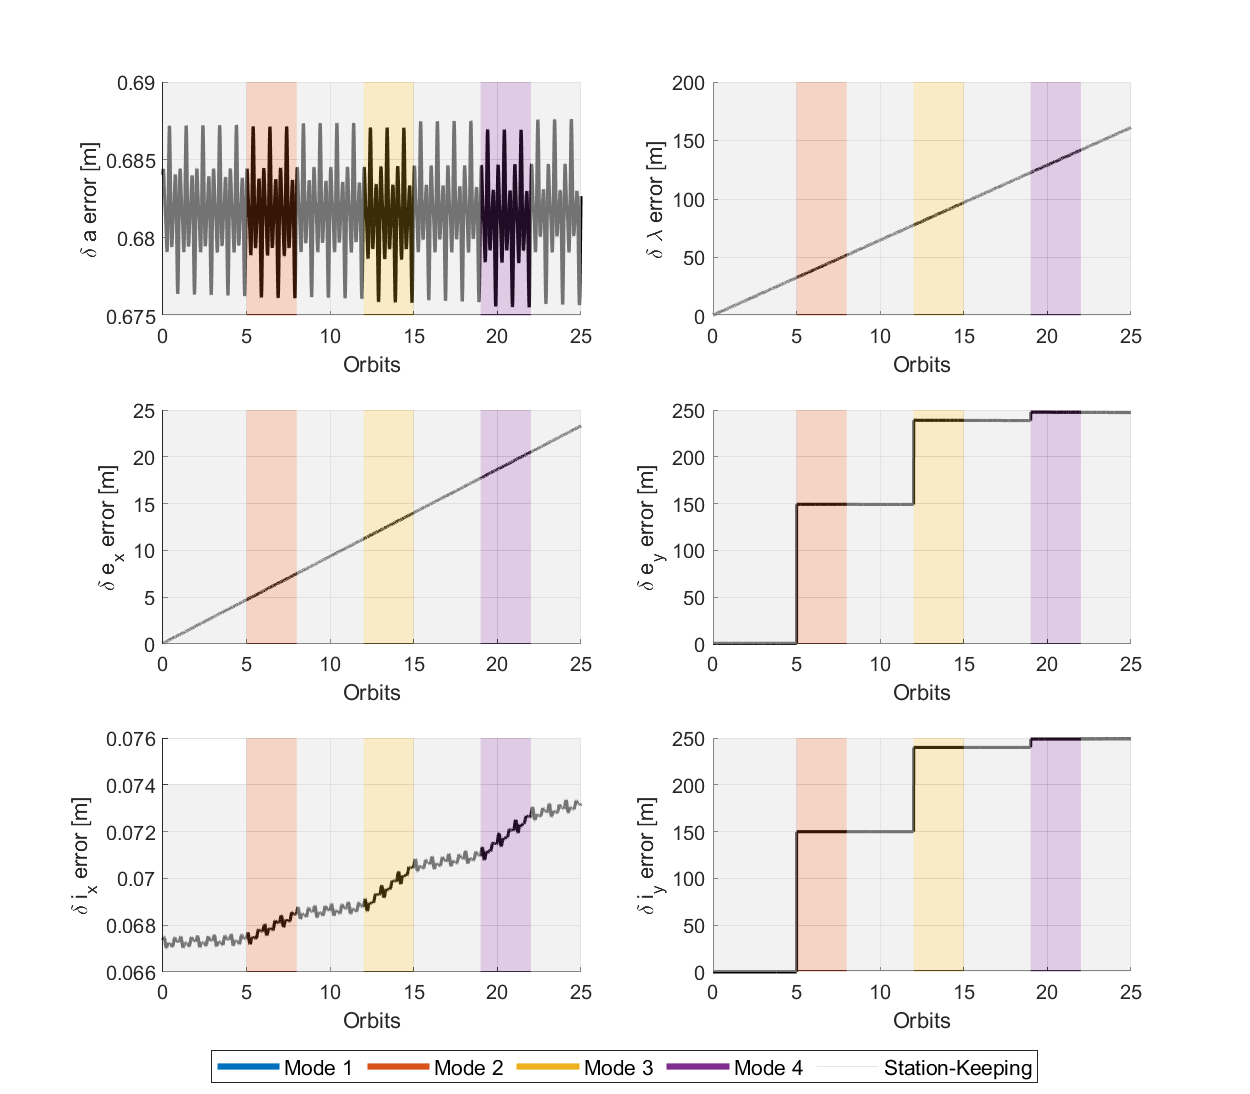
\includegraphics[width=0.75\linewidth]{sim/figures/PS6/ROE_error_over_time_modes_SV3.png}
    \caption{Tracking error between actual and desired ROE plotted for all modes in ROE time history, SV3}
    \label{fig:roe_error_time_modes_cont_SV3}
\end{figure}

Figure \ref{fig:delta_v_modes_cont_SV3} shows the delta-v magnitudes in the RTN directions throughout each control mode for SV3. By design, there are no radial burns. As expected, individual delta-v magnitudes are similar to impulsive ones in magnitude and are on the scale of mm/s. However, the cumulative delta-v magnitudes for each mode are much larger due to the nature of continuous control. In this implementation, continuous control is broken into impulsive like control for each time step. So, instead of a few delta-v's being applied for the entire control mode, as seen in impulsive control, continuous control has many delta-v's for extended periods of time. These delta-v's are also oscillating as they correct for tracking errors. These characteristics make continuous control exhibit much larger total delta-v than impulsive control. 

The magnitudes decrease in size as the desired change in ROE decreases throughout the modes. Additionally, there are more burns in the normal direction than in the tangential direction. This arises from the fact that inclination maneuvers are much more expensive than eccentricity maneuvers. Since each mode changes relative eccentricity and relative inclination by the exact same magnitude, the inclination maneuver is going to have to be larger. 
\begin{figure}[H]
    \centering
    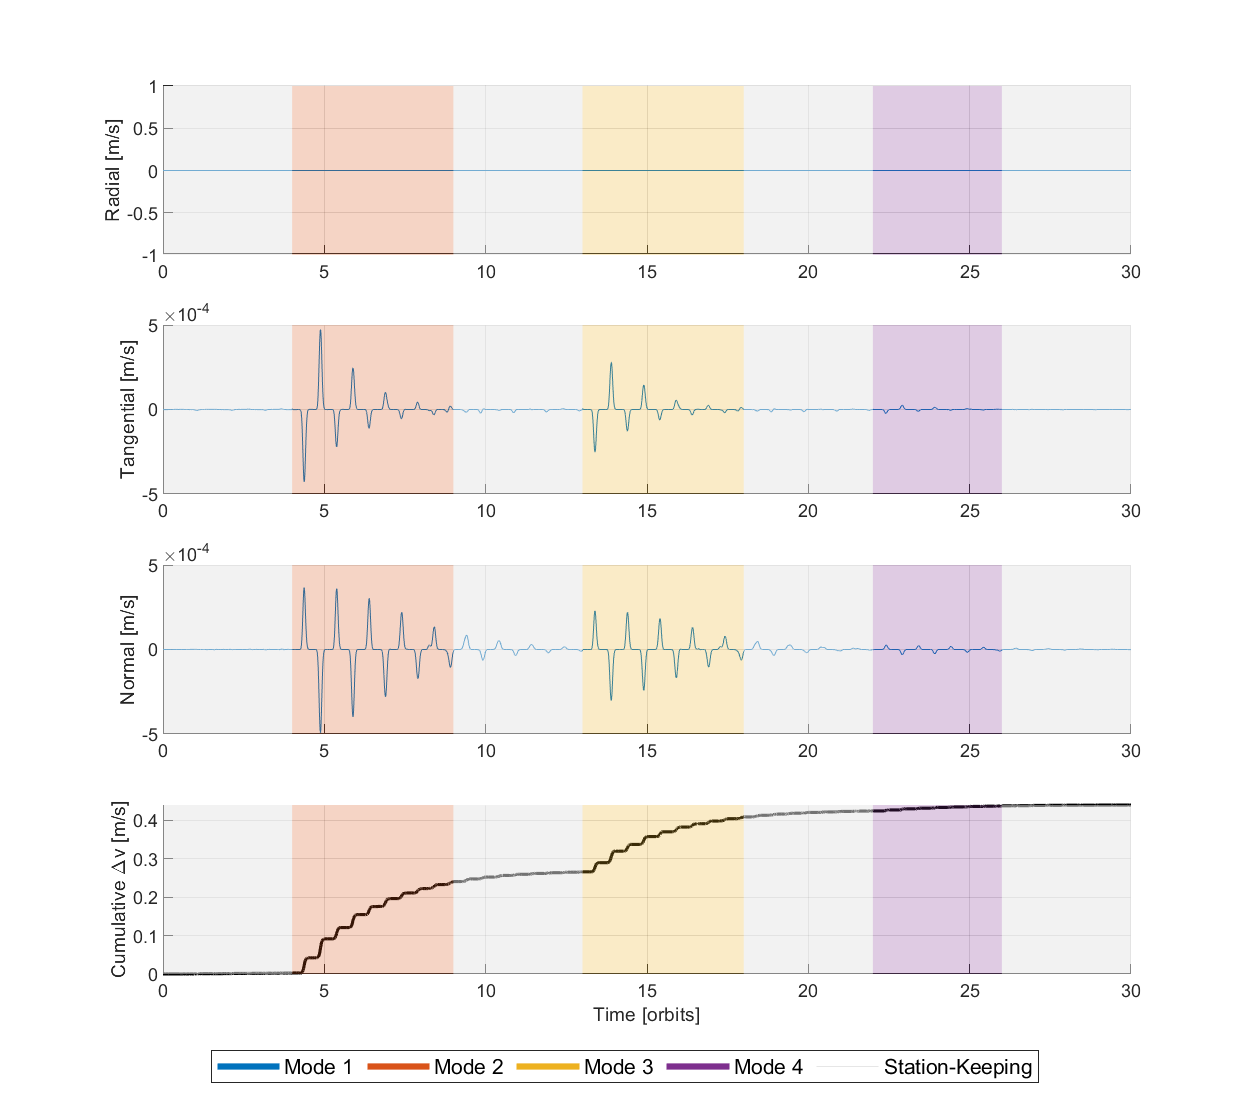
\includegraphics[width=0.75\linewidth]{sim/figures/PS6/delta_v_cumulative_timeline_modes_SV3.png}
    \caption{Actual delta-v of control maneuvers over time, SV3}
    \label{fig:delta_v_modes_cont_SV3}
\end{figure}

As a point of comparison, the theoretical delta-v lower bound can be calculated as follows:
\begin{align*}
\Delta v_{\text{ecc}} &= \frac{1}{2} \cdot n \cdot a \cdot \left\| \Delta \delta\vec{e} \right\| \\
\Delta v_{\text{inc}} &= n \cdot a \cdot \left\| \Delta \delta\vec{i} \right\| \\
\Delta v_{\text{lb}} &= \sqrt{\Delta v_{\text{ecc}}^2 + \Delta v_{\text{inc}}^2}
\end{align*}
Note that only changes in ROEs were in $\delta e$ and $\delta i$, which is why delta-v lower bound can be calculated as the norm of the along-track and cross-track delta-v's. 

Table \ref{tab:dv_comparison_continuous} compares the total delta-v with the theoretical lower-bound. The actual delta-v's were approximately 30 \% larger than the theoretical lower-bound for each mode. This is due to the nature of continuous control with frequent, oscillatory burns as mentioned previously. A greater total delta-v for continuous control is acceptable since a low-thrust engine, such as a Hall Effect Thruster, has much higher specific impulse than a higher-thrust engine, such as a cold-gas thruster, which would likely be used for impulsive control. That being said, the control strategy could be improved to better optimize delta-v and thus fuel usage through the introduction of constraints in the Lyapunov formulation and exploration of convex optimization. 
\begin{table}[H]
\centering
\begin{tabular}{|c|c|c|}
\hline
\textbf{Mode} & \textbf{Total }$\Delta v$ \textbf{(m/s)} & \textbf{Lower Bound (m/s)} \\
\hline
2 & 0.2377 & 0.1830 \\
3 & 0.1430 & 0.1098 \\
4 & 0.0132 & 0.0110 \\
\hline
\end{tabular}
\caption{Total delta-$v$ for continuous control compared with theoretical lower bounds for each maneuver mode}
\label{tab:dv_comparison_continuous}
\end{table}
